% The design space: 2 mass points x 3 gates x 2 personalization settings (12 cells), the two support-mask probes,
% the cells that coincide with existing methods, and the families outside the space (compiled to
% ../figures/fig_designspace.pdf by ../make_diagrams.sh). PRE blue, POST orange, as in the data figures.
% Cell (row, column, block) = (mass point, gate, personalization); the cell name is {post,pre}_{gate}_{off,on}.
\documentclass[tikz,border=1.5pt]{standalone}
\usepackage{amsmath,amssymb}
\usetikzlibrary{arrows.meta,positioning,fit,backgrounds,calc}
\definecolor{vblue}{HTML}{2A78D6}
\definecolor{vorange}{HTML}{EB6834}
\definecolor{ink}{HTML}{0B0B0B}
\definecolor{inktwo}{HTML}{52514E}
\definecolor{muted}{HTML}{8A8985}
\definecolor{exist}{HTML}{E4E3DF}
\definecolor{focus}{HTML}{E3EEFC}
\begin{document}
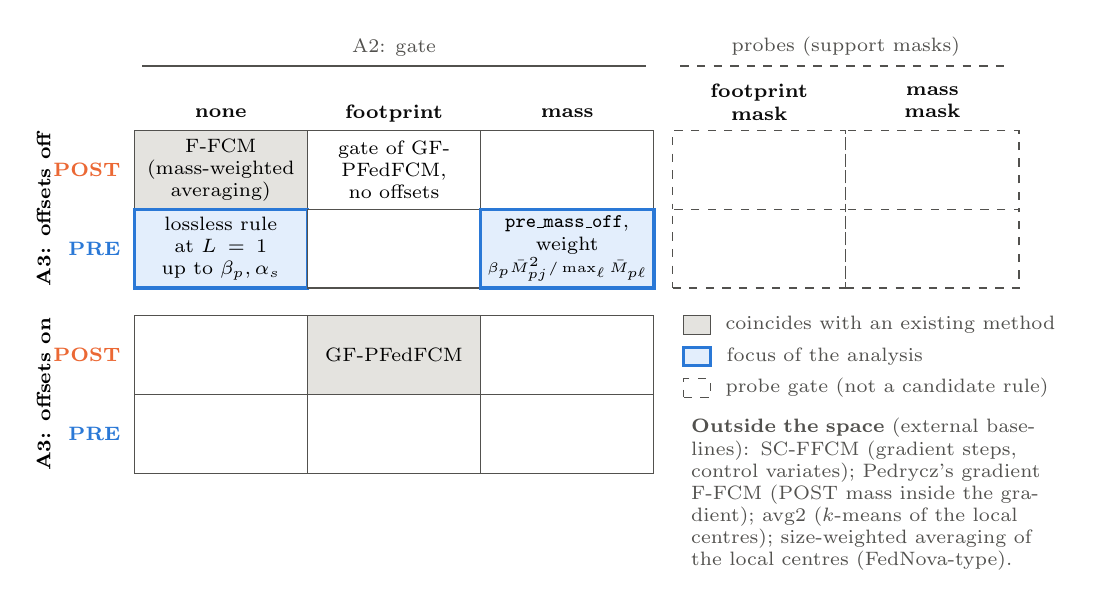
\begin{tikzpicture}[font=\scriptsize,
  cell/.style={draw=inktwo, line width=0.45pt, minimum width=2.2cm, text width=2.08cm, minimum height=1.0cm,
               align=center, inner sep=0.6pt, outer sep=0pt, fill=white},
  probe/.style={cell, dashed},
  focuscell/.style={cell, fill=focus, draw=vblue, line width=1.2pt},
  head/.style={font=\scriptsize\bfseries, text=ink, align=center, text width=2.1cm},
  rowlab/.style={font=\scriptsize\bfseries, align=right, anchor=east},
  note/.style={font=\scriptsize, text=inktwo, align=left}]
\def\W{2.2}\def\H{1.0}\def\X{0.95}
% ---------------- column heads (A2: gate), probes
\foreach \g/\x in {none/0, footprint/1, mass/2} {\node[head] at (\x*\W,0.72) {\g};}
\node[head] at (3*\W+\X*0.25,0.86) {footprint\\ mask};
\node[head] at (4*\W+\X*0.25,0.86) {mass\\ mask};
\draw[inktwo, line width=0.4pt] (-1.0,1.32) -- (2*\W+1.0,1.32) node[midway, above, text=inktwo] {A2: gate};
\draw[inktwo, line width=0.4pt, dashed] (3*\W+\X*0.25-1.0,1.32) -- (4*\W+\X*0.25+1.0,1.32)
      node[midway, above, text=inktwo] {probes (support masks)};
% ---------------- A3 off
\node[font=\scriptsize\bfseries, rotate=90] at (-2.25,-0.5*\H) {A3: offsets off};
\node[rowlab, text=vorange] at (-1.15,0) {POST};
\node[rowlab, text=vblue] at (-1.15,-\H) {PRE};
\node[cell, fill=exist] at (0,0) {F-FCM\\ (mass-weighted averaging)};
\node[cell] at (\W,0) {gate of GF-PFedFCM, no offsets};
\node[cell] at (2*\W,0) {};
\node[probe] at (3*\W+\X*0.25,0) {};
\node[probe] at (4*\W+\X*0.25,0) {};
\node[focuscell] at (0,-\H) {lossless rule at $L=1$ up to $\beta_p,\alpha_s$};
\node[cell] at (\W,-\H) {};
\node[focuscell] at (2*\W,-\H) {\texttt{pre\_mass\_off}, weight\\ {\tiny$\beta_p\bar M_{pj}^{2}/\max_\ell\bar M_{p\ell}$}};
\node[probe] at (3*\W+\X*0.25,-\H) {};
\node[probe] at (4*\W+\X*0.25,-\H) {};
% ---------------- A3 on
\def\Y{-2.35}
\node[font=\scriptsize\bfseries, rotate=90] at (-2.25,\Y-0.5*\H) {A3: offsets on};
\node[rowlab, text=vorange] at (-1.15,\Y) {POST};
\node[rowlab, text=vblue] at (-1.15,\Y-\H) {PRE};
\node[cell] at (0,\Y) {};
\node[cell, fill=exist] at (\W,\Y) {GF-PFedFCM};
\node[cell] at (2*\W,\Y) {};
\node[cell] at (0,\Y-\H) {};
\node[cell] at (\W,\Y-\H) {};
\node[cell] at (2*\W,\Y-\H) {};
% ---------------- key and families outside the space
\def\KX{3*\W-0.55}
\node[draw=inktwo, fill=exist, minimum width=0.34cm, minimum height=0.22cm] (k1) at (\KX,\Y+0.38) {};
\node[note, anchor=west] at ($(k1.east)+(0.06,0)$) {coincides with an existing method};
\node[draw=vblue, line width=1.2pt, fill=focus, minimum width=0.34cm, minimum height=0.22cm] (k2) at (\KX,\Y-0.02) {};
\node[note, anchor=west] at ($(k2.east)+(0.06,0)$) {focus of the analysis};
\node[draw=inktwo, dashed, minimum width=0.34cm, minimum height=0.22cm] (k3) at (\KX,\Y-0.42) {};
\node[note, anchor=west] at ($(k3.east)+(0.06,0)$) {probe gate (not a candidate rule)};
\node[note, anchor=north west, text width=4.6cm] at (\KX-0.2,\Y-0.68)
  {\textbf{Outside the space} (external baselines): SC-FFCM (gradient steps, control variates);
   Pedrycz's gradient F-FCM (POST mass inside the gradient); avg2 ($k$-means of the local centres);
   size-weighted averaging of the local centres (FedNova-type).};
\end{tikzpicture}
\end{document}
